\section{本章の概要}
本章では,開発したシステムの評価実験とその考察について述べる.
そして本研究では,学習者が座学における学習目標設定方法による学習と本システムのグラフデータ可視化機能を用いた学習目標設定方法による学習を比較し,
有用性を検証するための事前事後テストによる評価実験とアンケートによる利用評価実験を実施した.

\section{座学と比較した本システムによる学習の有用性検証実験}
実験では,基本情報技術者試験の午前試験\cite{gozen}を基にした,事前テスト事後テストによる座学と比較した本システムによる
学習の有用性を検証した.

\subsection{実験対象者}
実験対象者は,情報学科の学生と情報学科を卒業した大学院生(4年生:4名,修士1年生:7名,修士2年生:5名)の16名を実験協力者とした.
当学科では,3年生までにプログラミングは勿論ながら様々な情報学に関しての講義があるため,基本情報処理技術者試験の午前試験に関する知識も備えている.

\subsection{実験準備}
本実験を実施するにあたり,基本情報技術者試験の午前試験に関する事前テスト・事後テストを用意した.
学習教材としては事前テストに解説を付属させておりそれを学習教材とした.

事前テスト,事後テストはともに10点満点として,事前テスト・事後テストは同レベルの別の問題を使用した.
事前テストと事後テストはGoole From上で解答してもらった.
事前テストの内容を図\ref{fig:jizen1}~図\ref{fig:jizen6}に示す.
事後テストの内容を図\ref{fig:jigo1}~図\ref{fig:jigo6}に示す.
学習教材の例を図\ref{fig:kyozai1},図\ref{fig:kyozai2}に示す.

\begin{figure}[htbp]
\begin{center}
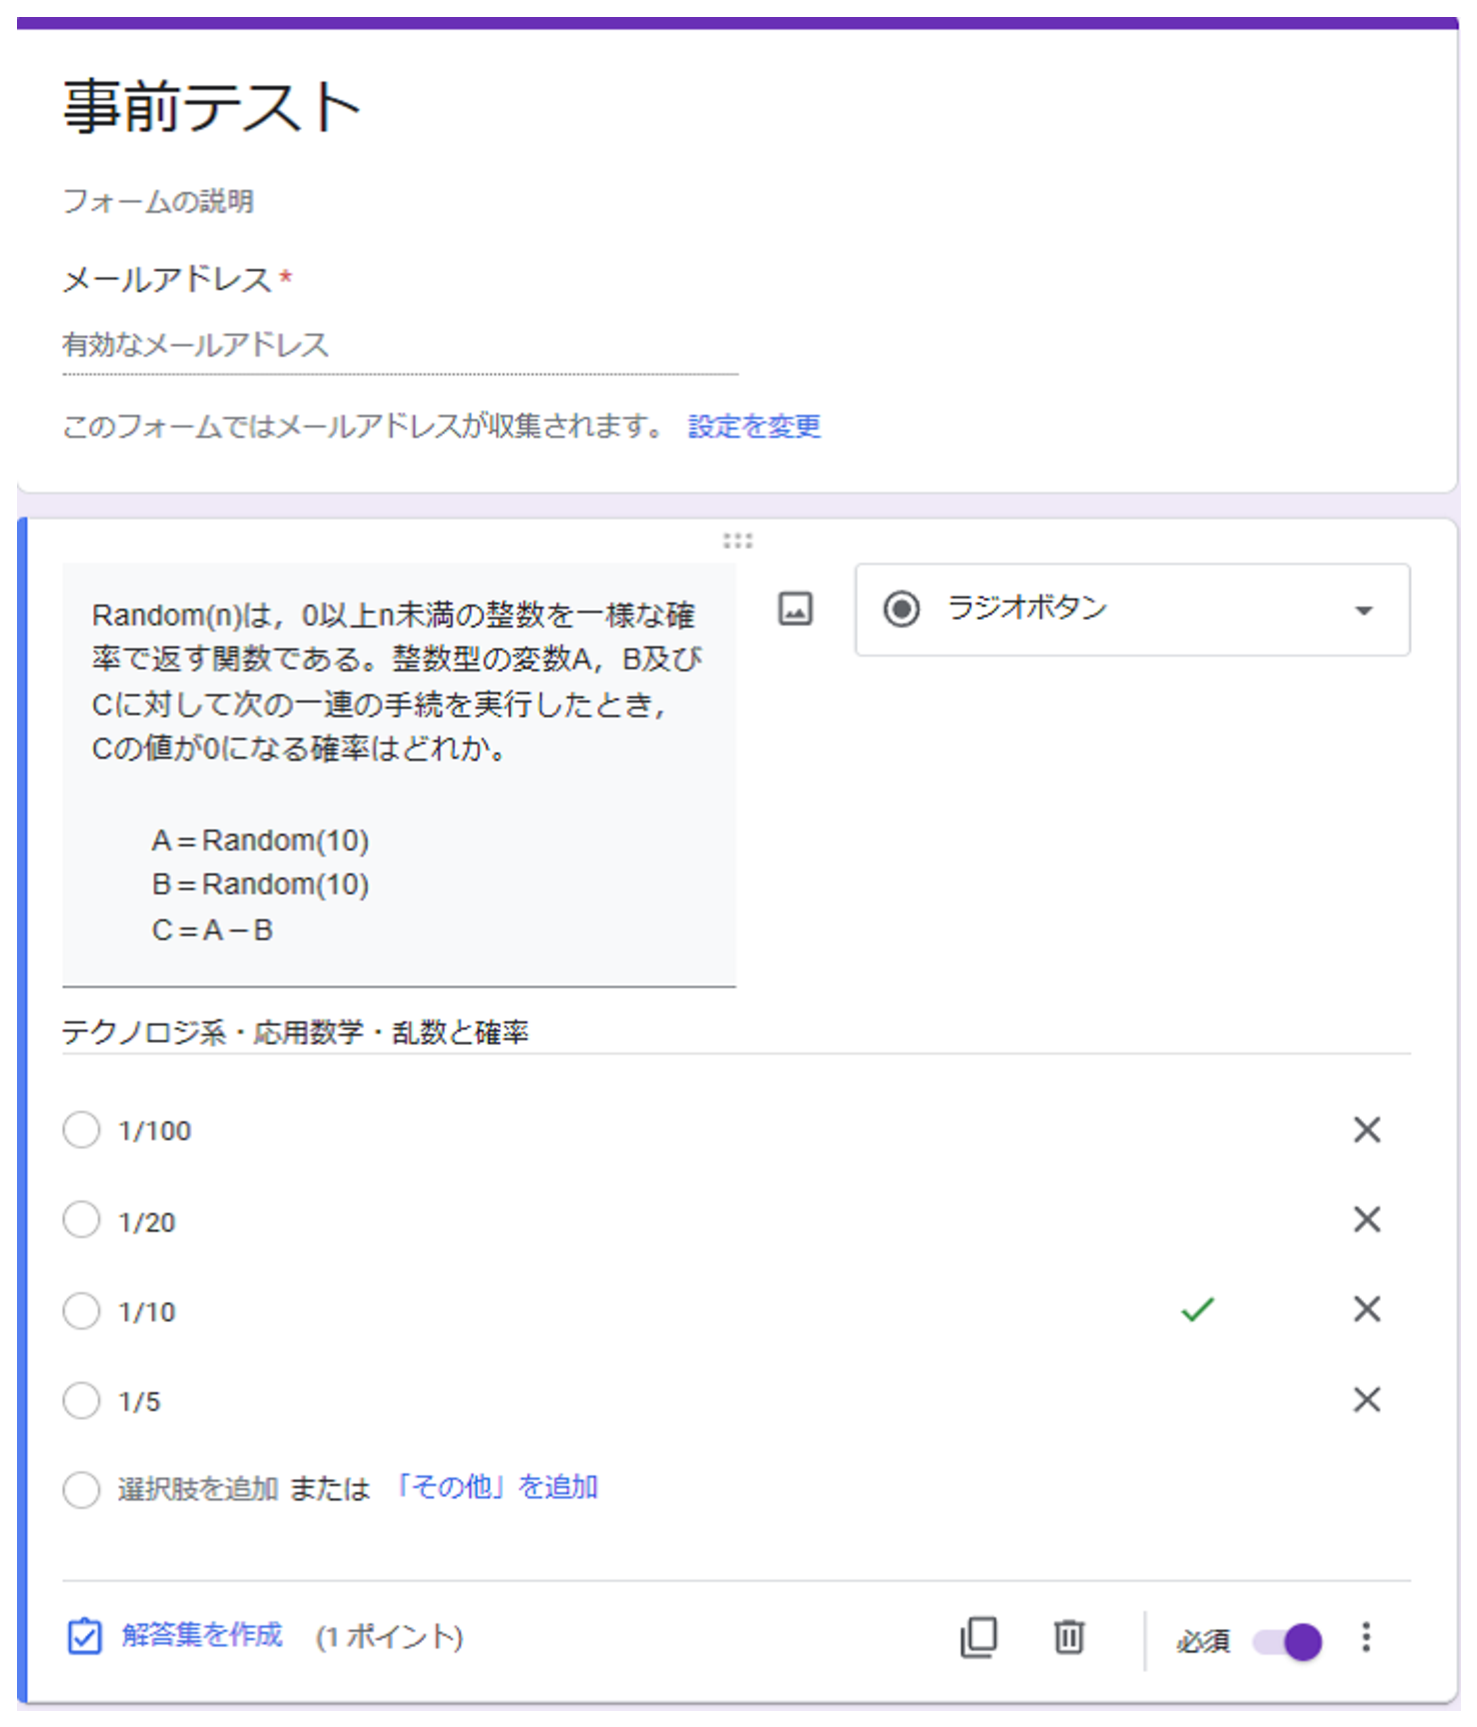
\includegraphics[width=13cm]{img/jizen1.eps}
\end{center}
\caption{事前テスト問題例1}
\label{fig:jizen1}
\end{figure}

\begin{figure}[htbp]
\begin{center}
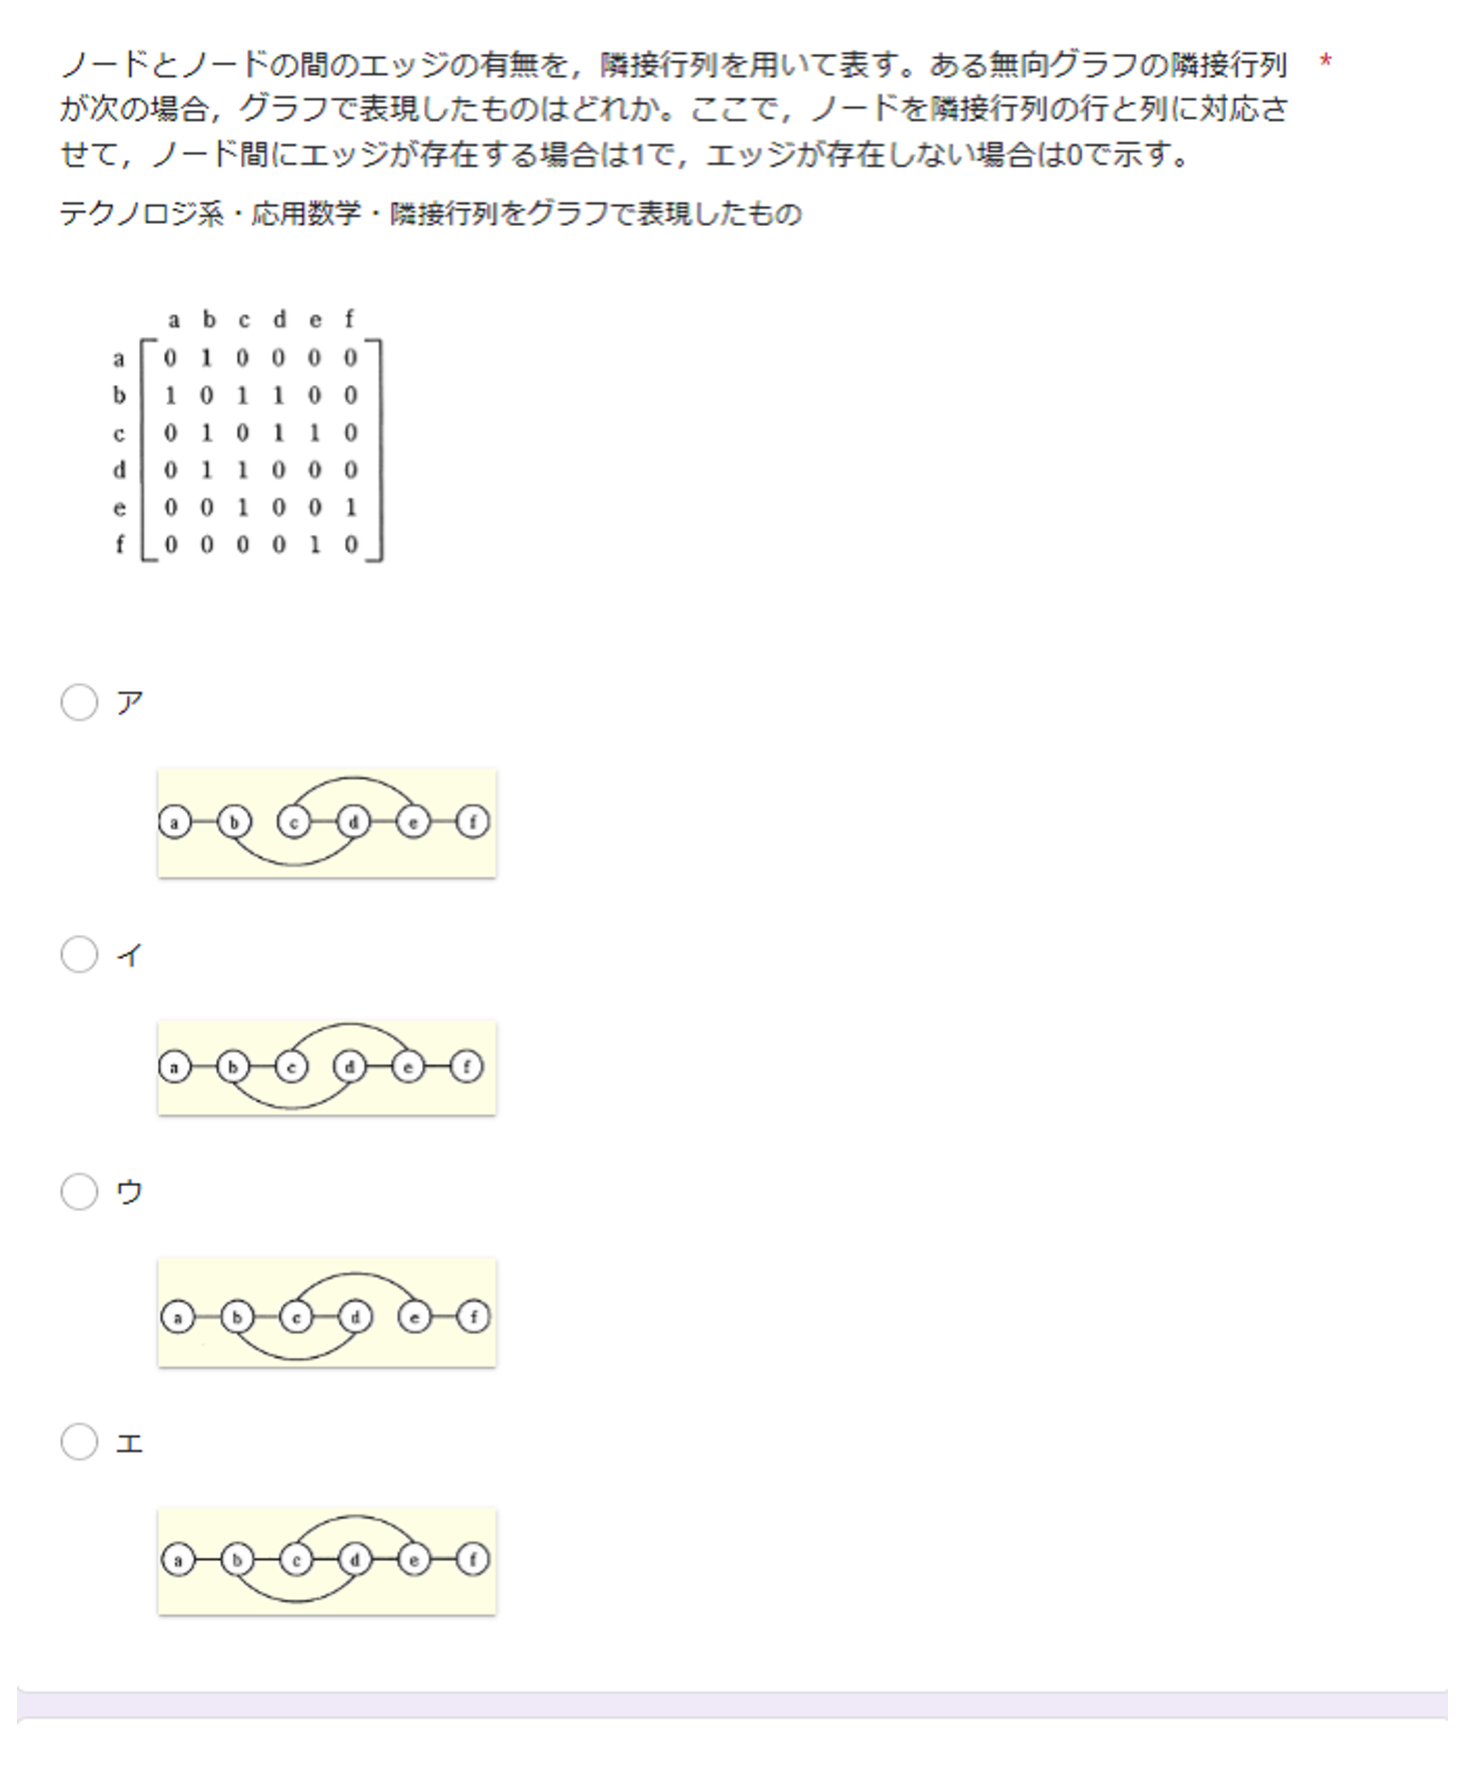
\includegraphics[width=16cm]{img/jizen3.eps}
\end{center}
\caption{事前テスト問題例2}
\label{fig:jizen3}
\end{figure}

\begin{figure}[htbp]
\begin{center}
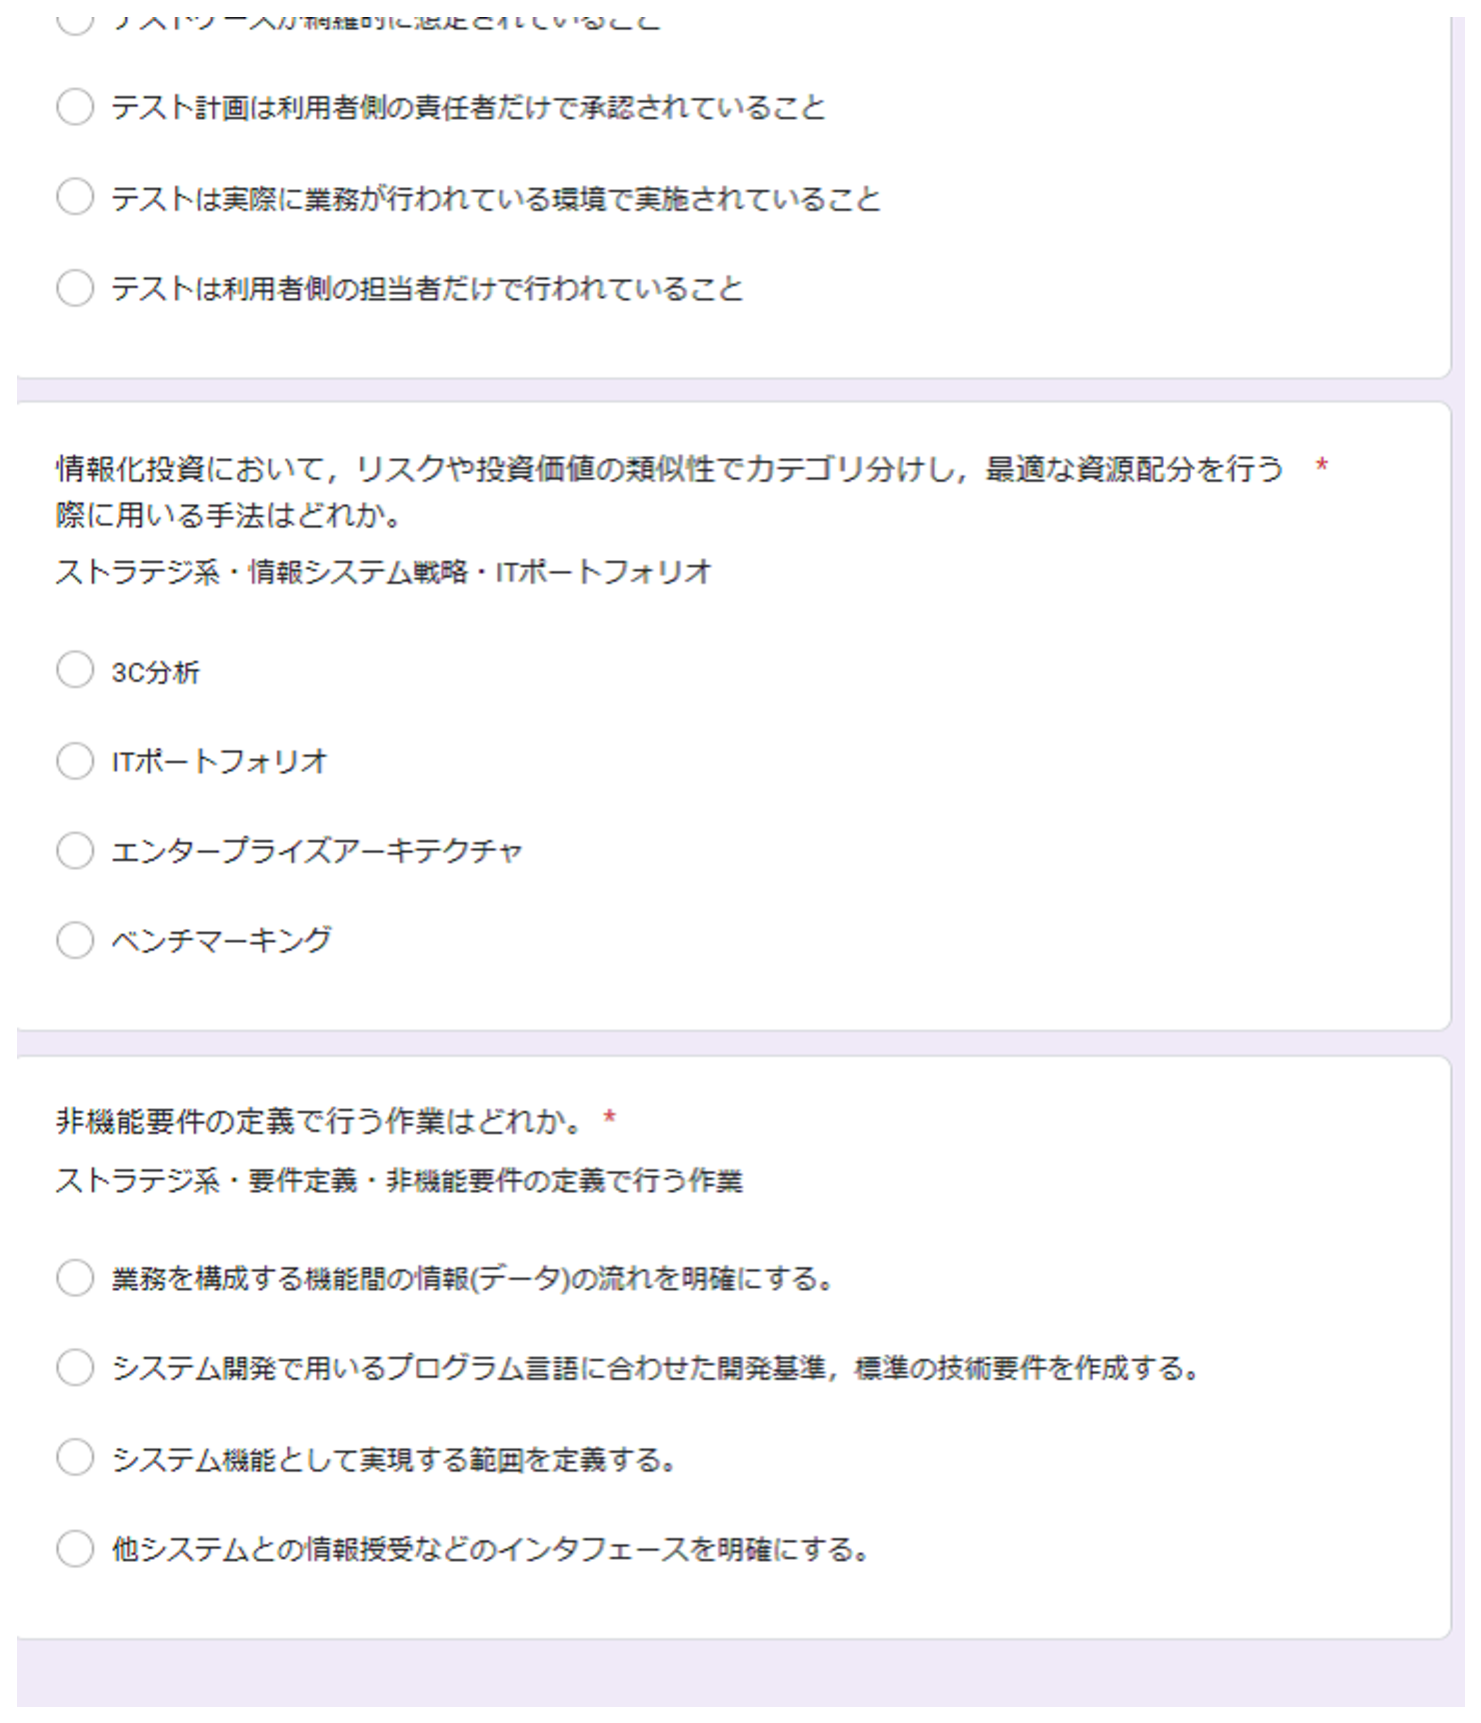
\includegraphics[width=16cm]{img/jizen6.eps}
\end{center}
\caption{事前テスト問題例3}
\label{fig:jizen6}
\end{figure}

\begin{figure}[htbp]
\begin{center}
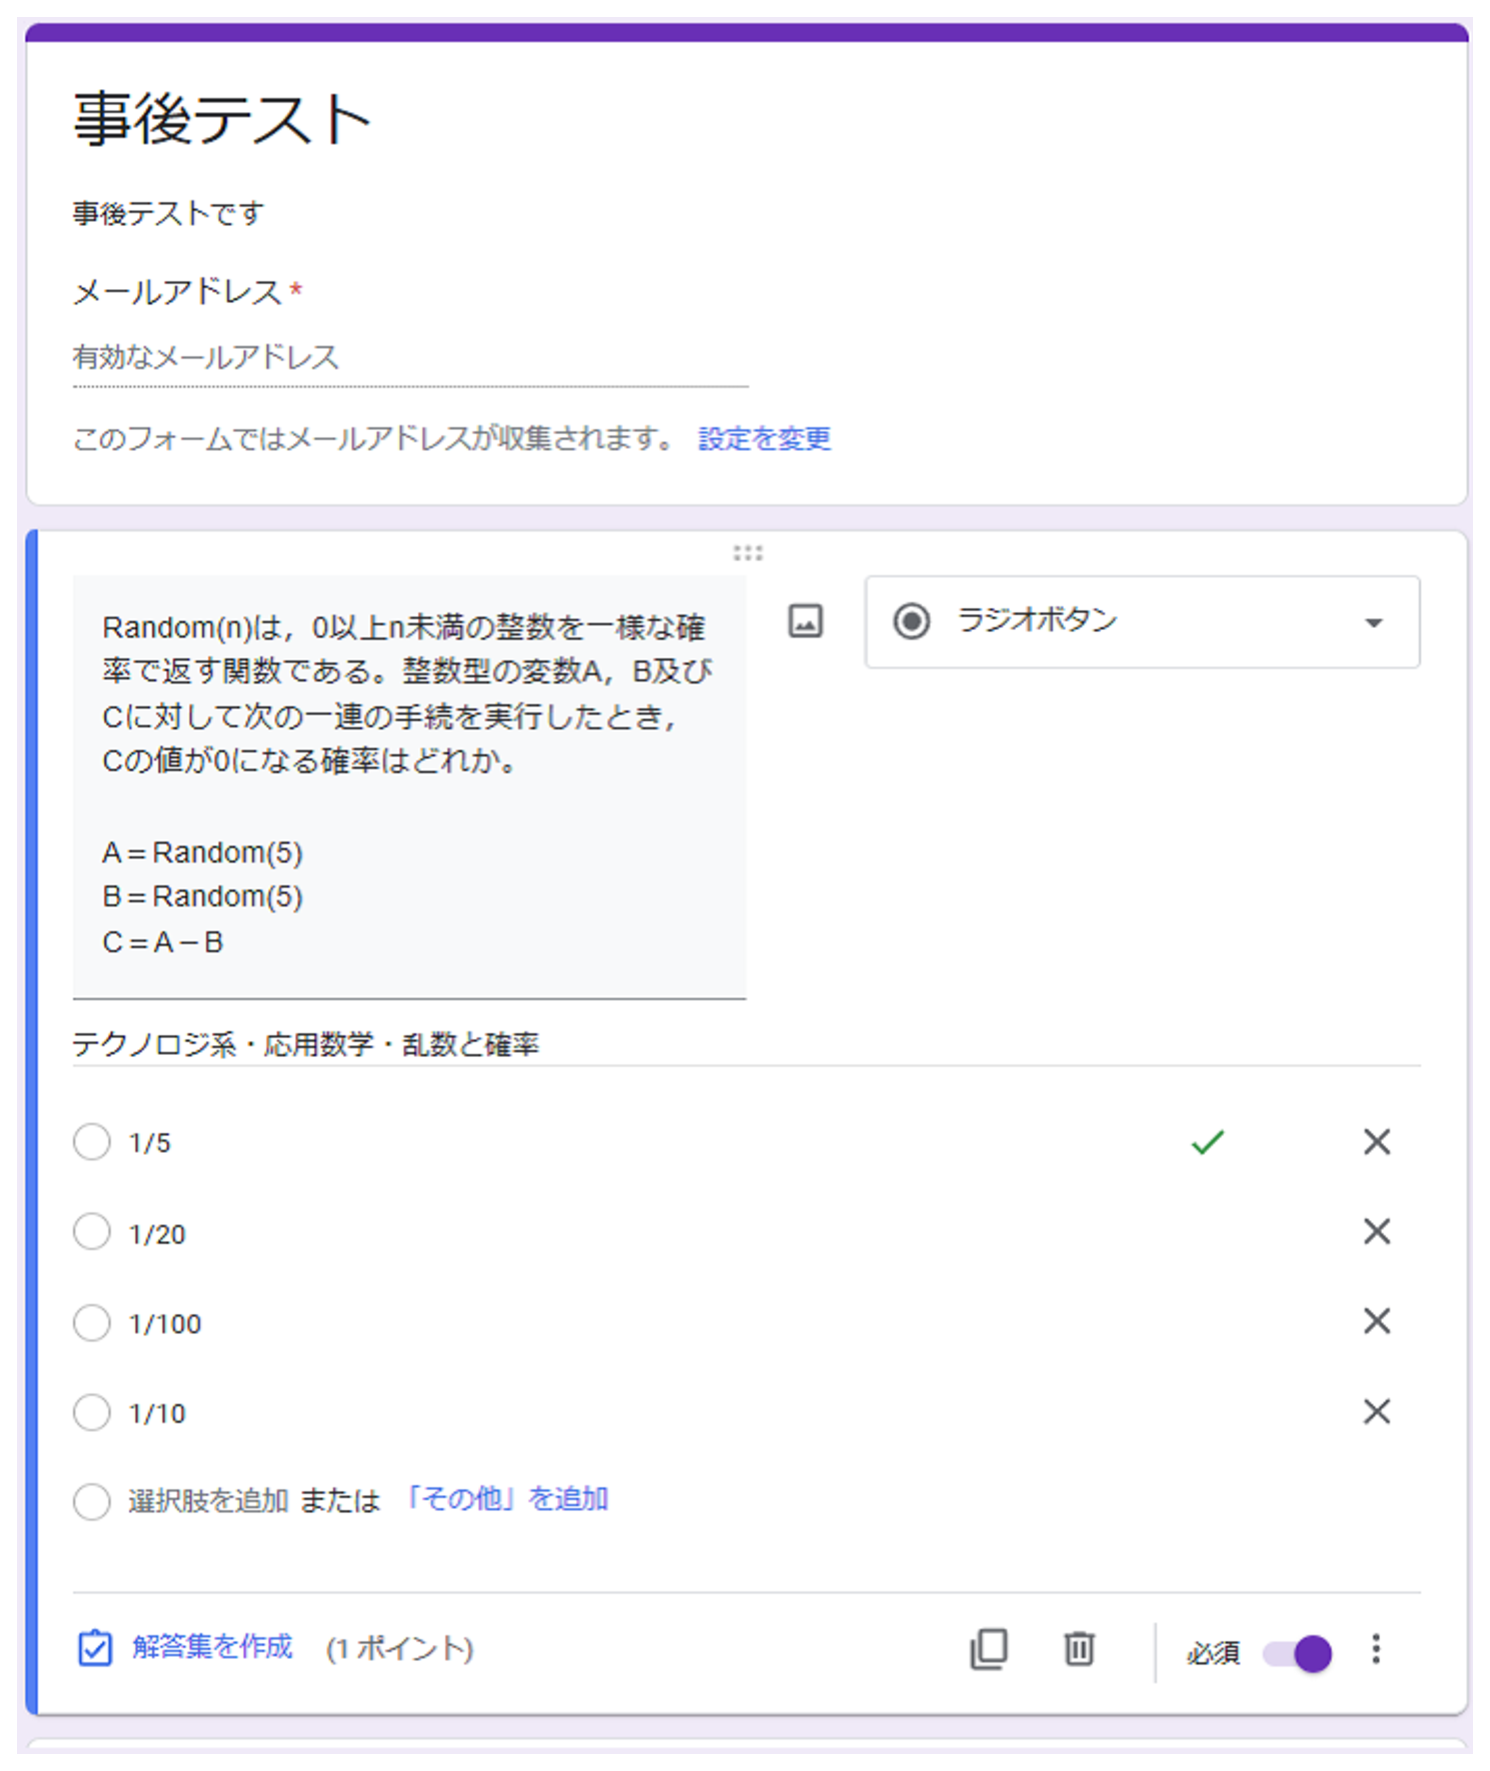
\includegraphics[width=16cm]{img/jigo1.eps}
\end{center}
\caption{事後テスト問題例1}
\label{fig:jigo1}
\end{figure}

\begin{figure}[htbp]
\begin{center}
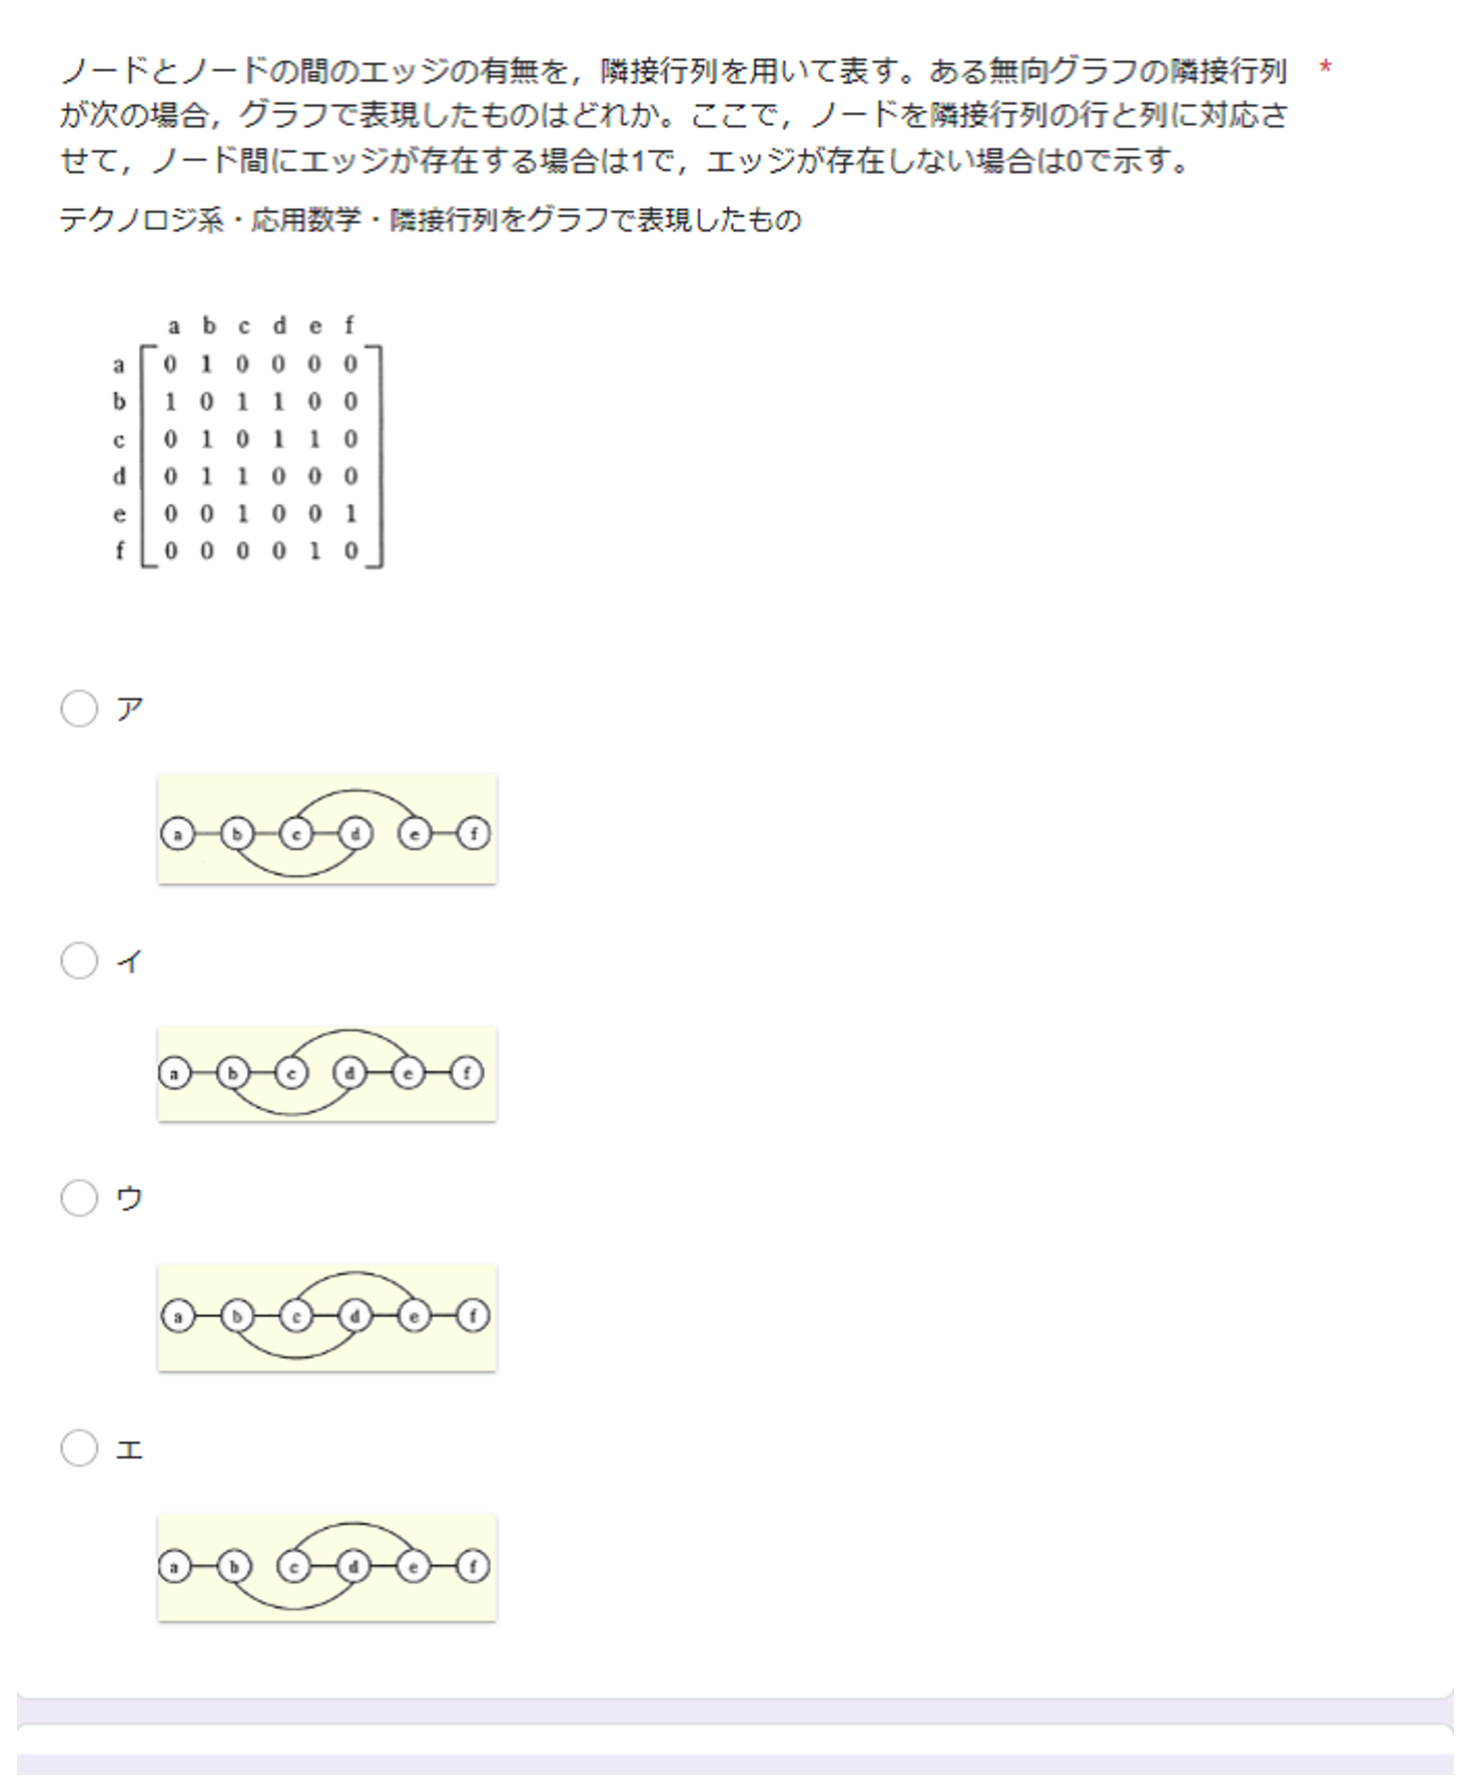
\includegraphics[width=16cm]{img/jigo3.eps}
\end{center}
\caption{事後テスト問題例2}
\label{fig:jigo3}
\end{figure}

\begin{figure}[htbp]
\begin{center}
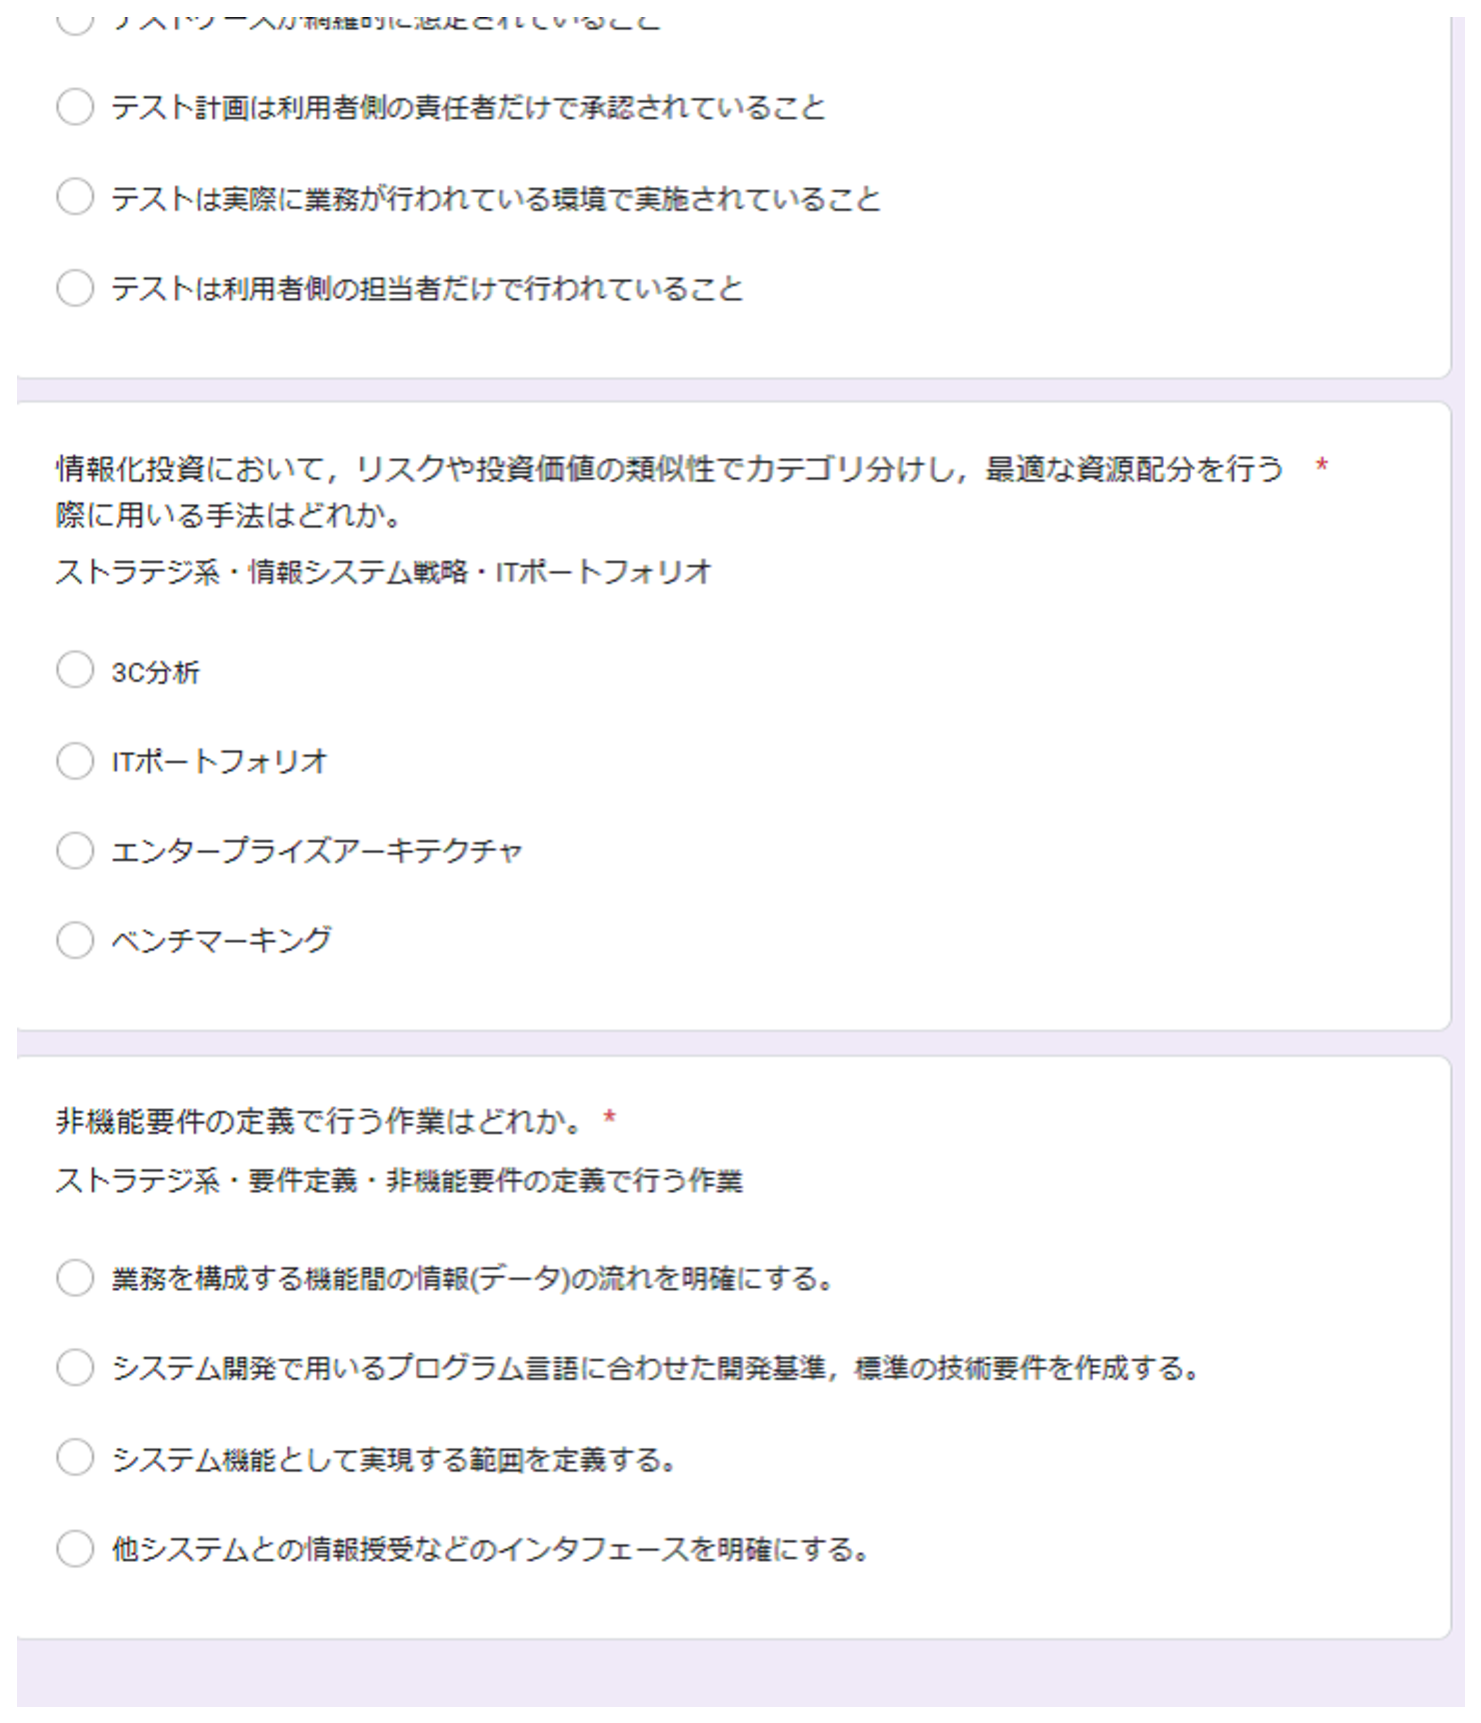
\includegraphics[width=16cm]{img/jizen6.eps}
\end{center}
\caption{事後テスト問題例3}
\label{fig:jigo6}
\end{figure}

\begin{figure}[htbp]
\begin{center}
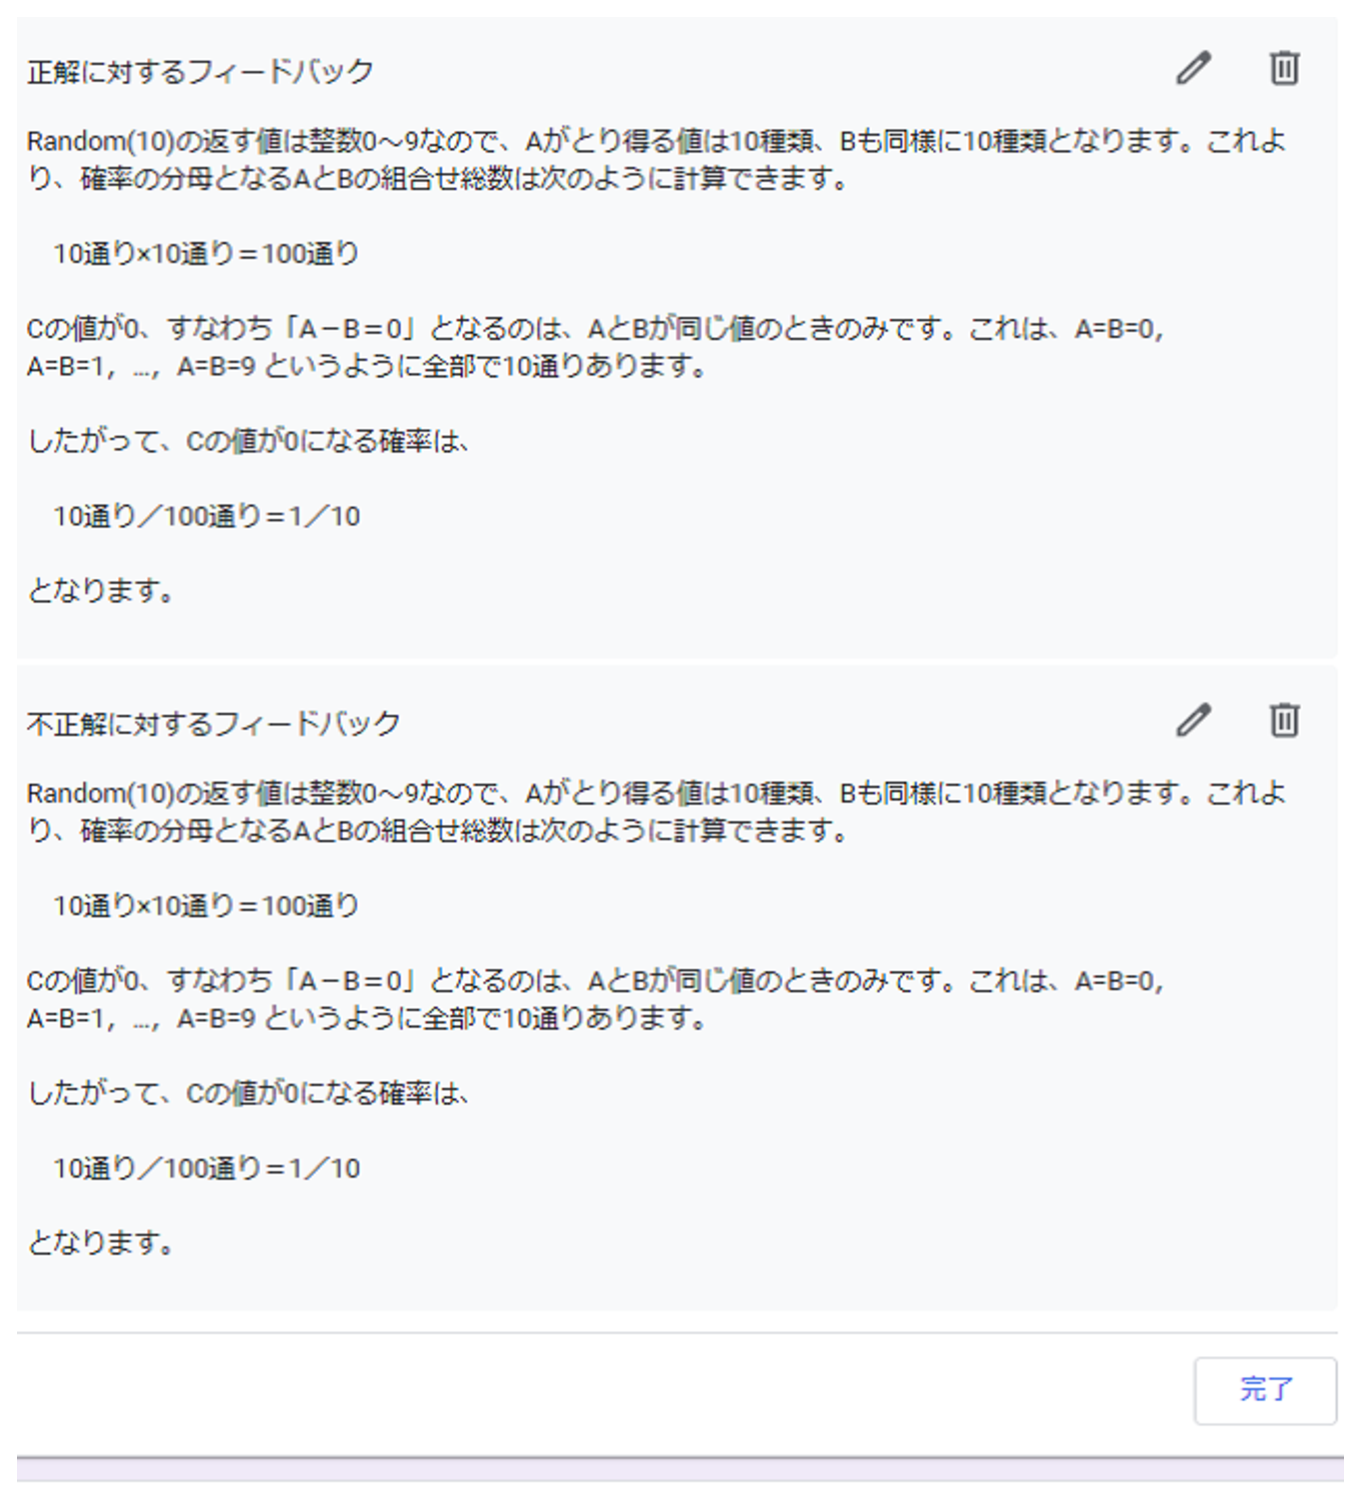
\includegraphics[width=16cm]{img/kyozai1.eps}
\end{center}
\caption{学習教材例1}
\label{fig:kyozai1}
\end{figure}

\begin{figure}[htbp]
\begin{center}
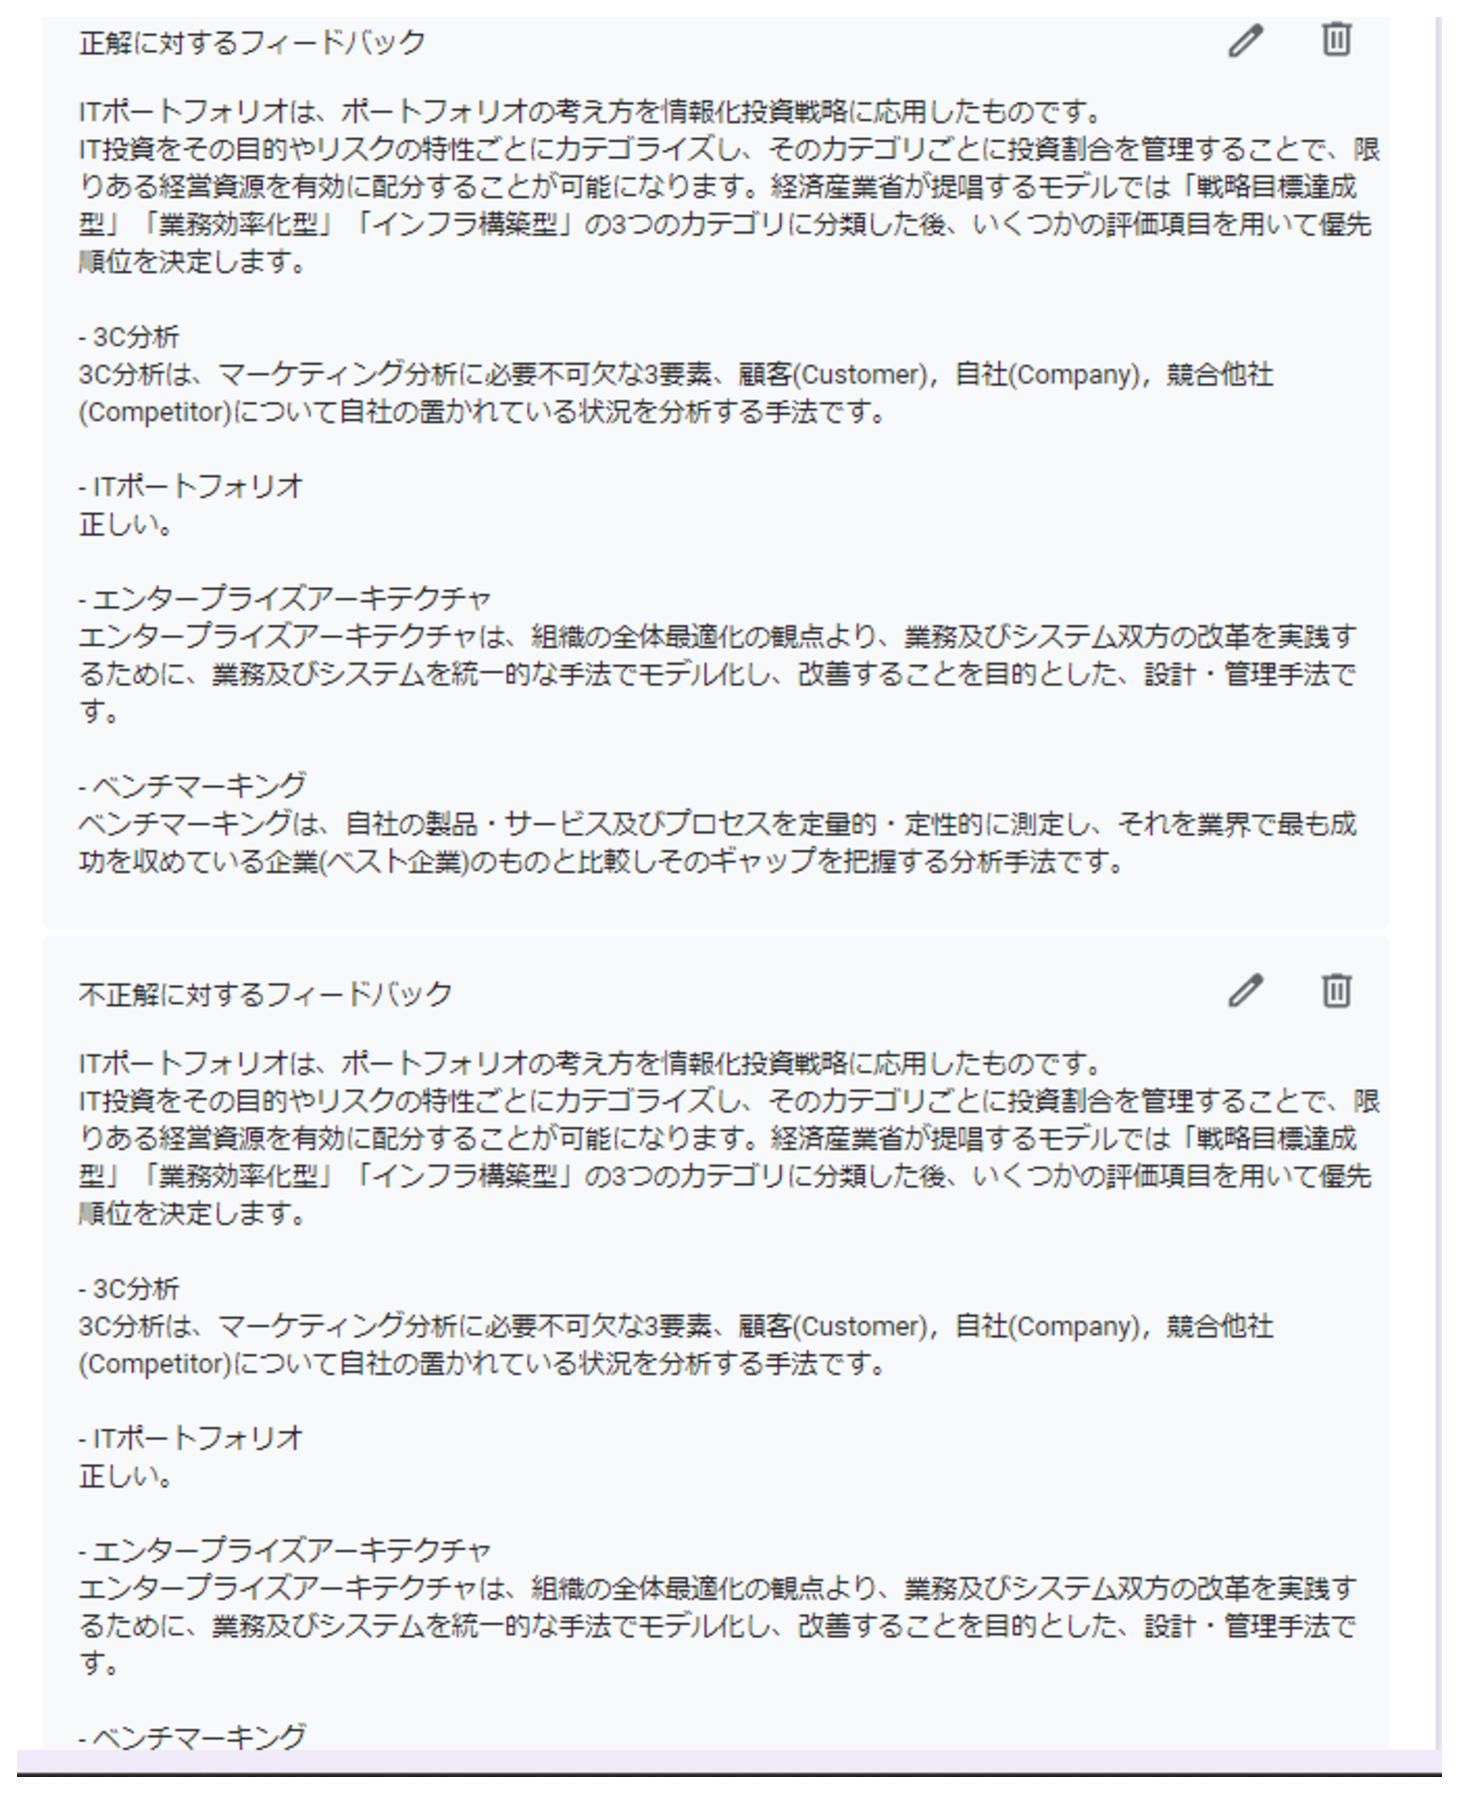
\includegraphics[width=16cm]{img/kyozai2.eps}
\end{center}
\caption{学習教材例2}
\label{fig:kyozai2}
\end{figure}

\subsection{実験手順}
まず,実験対象者16名に対して事前テストを実施した.
次に,事前テストの平均点が均等になるように8名ずつの2グループに分割した.
それぞれのグループをシステム利用者群,システム非利用者群とし,事前テストの結果と学習教材を基に各々のグループには学習目標を立ててもらい学習してもらった.
ただし,学習期間は3日間で合計3時間の学習時間とした.
両グループの学習終了後に実験対象者16名に事後テストを実施した.

\subsection{実験結果}
実験の結果を表\ref{tab:result1}に示す.表\ref{tab:result1}に示されるように,事後テストの点数の標準偏差は小さいため,実験対象者はシステム利用者群とシステム非利用者群ともに一定の水準の学習レベルに到達したと考えられる.
\begin{table}[tb]
    \centering
    \caption{実験結果}
    \label{tab:result1}
    \begin{tabular}{|c|c|c|c|c|c}
    \hline
     & \multicolumn{2}{c|}{事前テスト} & \multicolumn{2}{c|}{事後テスト} \\ \cline{2-5}
     & 平均 & 標準偏差 & 平均 & 標準偏差 \\ \hline
     本システム & 6.875 & 1.726 & 9.000 & 0.925 \\ \hline
     座学 & 6.875 & 1.552 & 7.625 & 1.597 \\ \hline
    \end{tabular}
\end{table}

事前テストと事後テストを受けた実験対象者全体の各問題における正答人数と誤答人数を図\ref{fig:result_jizen},図\ref{fig:result_jigo}に示す.


\begin{figure}[htbp]
\begin{center}
\includegraphics[width=18cm]{img/result_jizen.eps}
\end{center}
\caption{事前テストの全体結果}
\label{fig:result_jizen}
\end{figure}

\begin{figure}[htbp]
\begin{center}
\includegraphics[width=18cm]{img/result_jigo.eps}
\end{center}
\caption{事後テストの全体結果}
\label{fig:result_jigo}
\end{figure}

図\ref{fig:result_jizen}と図\ref{fig:result_jigo}内に示されている通り,誤答の多い問題は正答率が50\%未満の問題に限定すると,事前テストでは2問あったが事後テストではなくなっていることからも,実験対象者は本システムを利用した学習と座学でのみ学習した者たち共に,点数の上昇に限らず,知識を偏りなく習得できていることが確認できる.
また,表\ref{tab:result1}より,座学すなわちシステム非利用者群の平均点が0.75点増えているのに対し,本システム利用者群の平均点は2.125点上昇している.

加えて事前テストと事後テストにおけるt検定の結果を図\ref{fig:tcheck}に示す.
\begin{figure}[htbp]
\begin{center}
\includegraphics[width=18cm]{img/tcheck.eps}
\end{center}
\caption{t検定の結果}
\label{fig:tcheck}
\end{figure}
t検定では帰無仮説を「事前テストと事後テストの平均点は等しい」,対立仮説を「事前テストと事後テストの平均点は等しくない」,有意水準を0.05とした.
図\ref{fig:tcheck}から帰無仮説は棄却され,事前テストと事後テストの平均点は有意に異なることが分かった.
これは表\ref{tab:result1}と併せて考えるとシステム利用者群の平均点がシステム非利用者群と比べ明らかに点数の伸びが高い点から,本システムにおける学習目標設定方法が有意に作用した可能性が挙げられる.

以上の結果から,座学で学習したシステム非利用者群と比較して,本システムを利用して学習したシステム利用者群の方がより高い点数が得られたことが確認できた.

\newpage

\section{本システムの利用評価実験}
最後に本システムの利用評価実験を実施した.
実験対象者は座学と比較した本システムによる学習の有用性検証実験に参加した実験対象者16名全員に対してアンケートによる利用評価実験を行った.
利用評価実験で使用したアンケートは1~5の5段階評価で実施し,最後に自由記述欄を設けた.

アンケート結果を図\ref{fig:ank}に示す.

\begin{figure}[htbp]
\begin{center}
\includegraphics[width=18cm]{img/ank.eps}
\end{center}
\caption{アンケートの結果}
\label{fig:ank}
\end{figure}

アンケート結果から「事前テストの主観的問題難易度はどうでしたか」,「事後テストの主観的問題難易度はどうでしたか」という設問に対して,両群ともに数値が低く,問題難易度が低いと認識していたようである.
「事前テストにおける得点の割合は全体を通してどの程度あると思っていましたか」,「事後テストにおける得点の割合は全体を通してどの程度あると思っていましたか」という設問でも,両群ともに事前テストでは7割程度,事後テストでは8割程度得点出来ていると認識していたようである.
「事前テストの主観的得点と実際に返却された得点はどの程度離れていましたか」という設問に対しても両群ともに同じ割合分ギャップを感じていたようである.
一方「事後テストの主観的得点と実際に返却された得点はどの程度離れていましたか」という設問に対してシステム非利用者群は2.3,システム利用者群は1.5と0.8もの差が開いている.
このことからシステム利用者群はシステム非利用者群と比べて,自分の主観的学習理解度と実際に返却された学習理解度に差がなかったことが表されている.
すなわち,システム利用者の方がシステム非利用者と比べて,学習者自身の学習内容に対する主観的理解度と客観的理解度に差がなかったことが分かった.
この結果から,システム利用者群は正しく自身の学習進行度を理解できていたため,表\ref{tab:result1}で示されたようにシステム非利用者群より事後テストの得点が上昇していたのではと考えられる.

\section{考察}
座学と比較した本システムによる学習の有用性検証実験では,事前テストと事後テストの平均点がシステム利用者群のほうがシステム非利用者群より良い結果となり,t検定からも両群の平均には有意な差があることが分かった.
利用評価実験では,事前事後テストの主観的難易度は両軍ともに同程度と感じていたが,システム非利用者群に比べてシステム利用者群は学習者自身の学習内容に対する主観的理解度と客観的理解度に差がなかったことが分かった.
以上の実験の結果から座学による学習の学習目標設定方法と比べ,本システムを利用した学習目標設定方法のほうが学習者自身が学習内容の構造的理解と,主観的理解度と客観的理解度に差が付きづらいため,より正確な学習目標設定支援を行えることが分かった.
一方,本実験ではシステム非利用者群に対して本システムを用いないコンセプトマップ作成を用いた学習を実施していないため,今後の課題として,本システムを用いないコンセプトマップを用いた学習方法における学習目標設定方法と本システムを用いた学習目標設定方法の比較を実施する必要がある.